\documentclass[12pt]{article}

\usepackage{graphicx}

\graphicspath{{imagenes}}

\title{Manual OpenFoam}
\author{}

\begin{document}
\maketitle

\section{IncompressibleVoF}

Para poder facilitarnos el uso de IncompressibleVoF importaremos el ejemplo de "Breaking of a Dam" alabrir la terminal cambiar al siguiente directorio run/user/OpenFoam escribir lo siguiente: \\
cp -r \$FOAM\_TUTORIALS/incompressibleVoF/damBreakLaminar.

\subsection{Por deinir}
Primero chequemos los archivos que obtenemos al copiar la carpeta.\\
\begin{figure}[h]
  \centering
  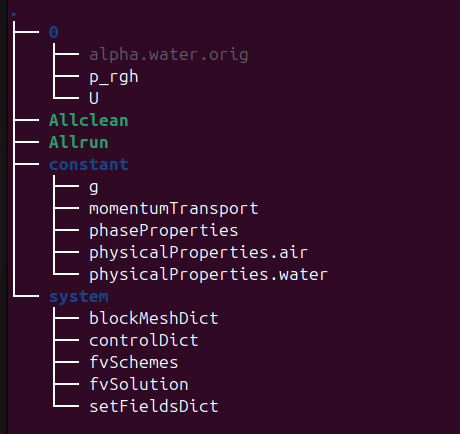
\includegraphics[width=0.5\linewidth]{tree-dambreak.png}
  \caption{Archivos de Dam Break Laminar}
\end{figure}

El primer archivo que vamos a editar es System/blockMeshDict en este esta dividido en tres partes: vertices, blocks y boundary.\\
En el primero pondremos todas los vertices de las caras de nuestro mesh con este formato "(x y z)" al acabar de colocar los puntos estos estaran enlistados comenzando por el 0 en relacion a su aparicion en el codigo, despues tenemos blocks en esta parte pondremos los bloques estos estan definidos por los puntos y para colocarlo tenemos que poner lo siguiente hex (p1 p2 p3 ... p8) (a b c) los 8 puntos deben de estar colocados de tal manera que si hay una arista entre los puntos deben estar uno siguiente del otro en la lista y el a, b y c es como queremos dividir al bloque y en boundary tenemos que definir las paredes de los bloques en este tenemos distintos tipos de maneras de definir las paredes:\\


\begin{itemize}
  \item type wall: este tipo nos permite que las paredes sean solidas dentro de los cubos 
  \item type patch:  este tipo nos permite la entrada y salida del liquido y este no aporta ninguna informacion sobre el la pared
  \item type symmetryPlane:  este tipo permite replicar lo que pasa en el plano
  \item type empty:  este tipo nos permite poder modelar en 2d o 1d ya que el sistema no tiene que solucionar para esas paredes

\end{itemize}
Al determinar las paredes podemos agrupar las distintas caras si tienen el mismo tipo o si cumplen alguna propiedad particular la cual sera importante despues en el modelo a esto se le llama boundaryField.\\

Para verificar como quedo el mesh podemos usar el comando blockMesh y paraFoam, lo que va a haacer blockMesh es compilar el codigo y paraFoam te va a dar un visualizador para ver el mesh\\

\begin{figure}[h]
  \centering
  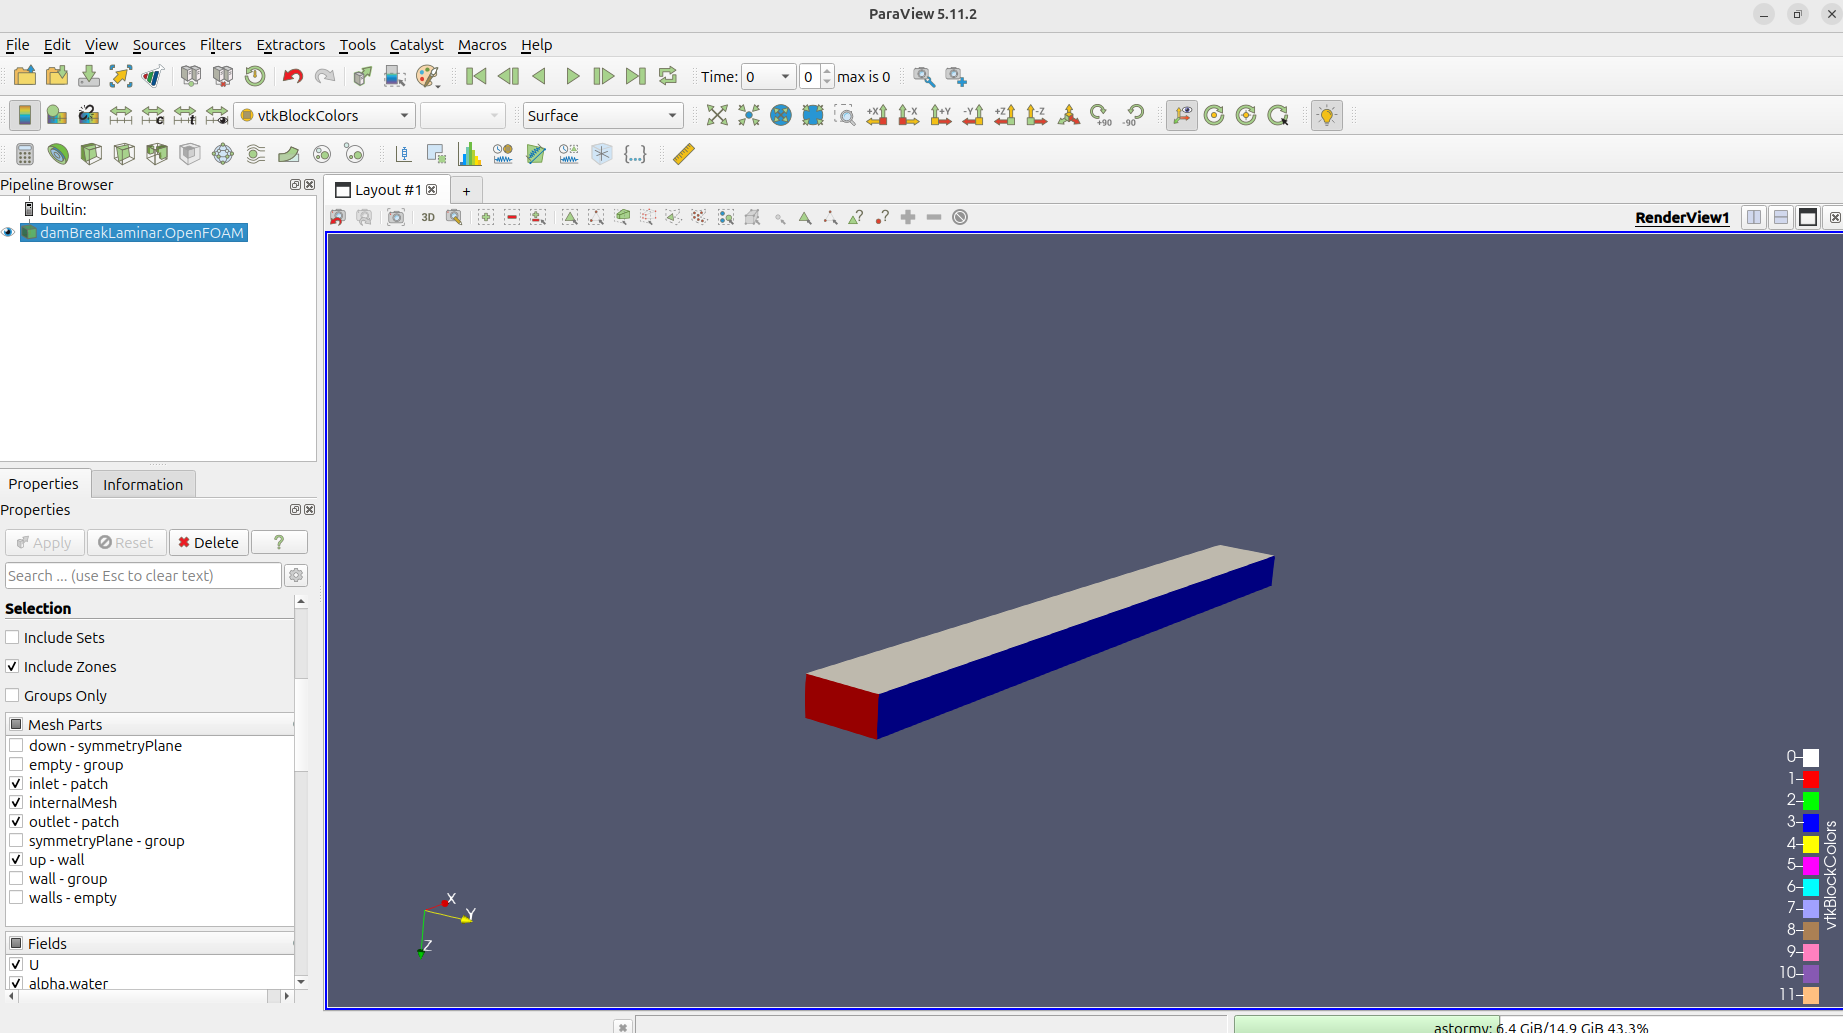
\includegraphics[width=0.9\linewidth]{modelo_3d.png}
  \caption{modelo 3d}
\end{figure}

Ahora vamos a editar las condiciones iniciales del sistema. Estas estan en la carpeta 0, comencemos con U este archivo tiene las velocidades del agua en las caras del sistema a esto se le llama boundaryMesh los tipos que se les puede asignar son los siguientes: \\

\begin{itemize}
  \item fixedValue: en este podemos poner la velocidad en la cual entra el fluido mediante agregarle en la linea de abajo value uniform(x y z) y el x y z es la velocidad en esa direccion 
  \item zeroGradient: este tipo obtiene la velocidad de una celula anterior a este y es usualmente usado para las caras por donde sale el fluido
  \item symmetryPlane: este tipo replica lo que pasa del otro lado del plano
  \item noSlip: este te permite obtener paredes que no resbalen 
  \item slip: permite que el fluido resbale por la cara seleccionada
  \item empty: este no agrega nada al modelo
\end{itemize}

Tambien en 0 tenemos el archivo p\_rgh en el cual tenemos la presion hidroestatica aqui podemos modificar los tipos de boundaryField este tiene los mismos tipos que el archivo U menos slip y noSlip a parte agregamos otro que es fixedFluxPressure que es una presion fija determinada por el sistema.\\

Con esto solo quedaria checar las propiedades fisicas del aire y del agua estos archivos estan en la carpeta constant
podemos modificar la viscosidad(nu) y densidad(rho) del liquido y del aire en los archivos physicalProperties.water y physicalProperties.air respectivamente
Tambien queda modificar las phaseProperties en las cuales definimos cuales son las fases del liquido con phases(water air) y en este tenemos sigma que es el coheficiente de tension superficial\\

Ahora los siguientes archivos que agregemos o que modifiquemos sera en relacion a si el tenemos un flujo laminar o turbulento\\

\subsection{Flujo Laminar}

Para flujo laminar como el ejemplo que estamos usando ya usa este modelo solo mostraremos en donde este modelo se define\\
Abriremos la carpeta constant y el archivo momentumTransport en este podemos ver el simulationType en el cual esta laminar

\subsection{Flujo Turublento}
Para flujo turbulento tenemos que modificar el archivo constant/momentumTransport y en simulationType poner RAS esto significa Reynolds-Averaged Simulation abajo de este pondremos que usaremos el modelo kEpsilon y que tiene turbulencia\\

\begin{figure}[h]
  \centering
  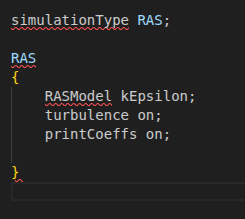
\includegraphics[width=0.3\linewidth]{ras_file.png}
  \caption{RAS formato}
\end{figure}

tendremos que agregar estos archivos en la carpeta 0 k, nut y epsilon.\\
Comencemos con k en esta tendremos que poner los boudaryField y en estos podemos difinir la energia kinetica del sistema en el cual tenemos las siguientes opciones para definir las paredes

\begin{itemize}
  \item fixedValue: a este le asignamos un valor fijo en la parte de abajo
  \item inletOutlet: es para cuando la direccion del flujo es desconocida
  \item symmetryPlane
  \item zeroGradient: es cuando 
  \item empty 
\end{itemize}

Ahora chequemos epsilon este es la relacion de disipacion de la energia kinetica y tiene los mismos valores que k\\ 

Por ultimo nut

\subsection{Agregar Funciones de Medicion}

En system/controlDict al final podemos agregar funciones mediante definir functions y probes de la siguiente manera y dentro de probes podemos definir lo que queremos medir del sistema

\begin{figure}[h]
  \centering
  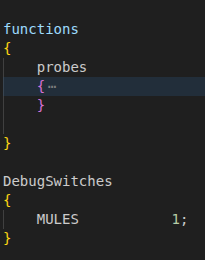
\includegraphics[width=0.4\linewidth]{funciones.png}
  \caption{Funciones de medicion}
\end{figure}

Dentro de probes nosotros queremos medir la presion, entonces haremos lo siguiente:
primero definiremos el campo que queremos medir en este caso es la presion que esta en el archivo p\_rgh y en particular la queremos medir en en ciertos puntos y estos puntos los colocamos en probeLocations de esta manera hacemos las cosas 

\begin{figure}[h]
  \centering
  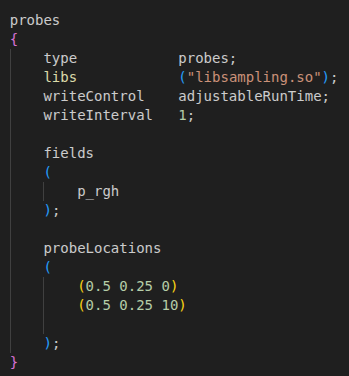
\includegraphics[width=0.4\linewidth]{probes_function.png}
  \caption{Funcion de presion}
\end{figure}

\subsection{Ejecucion del Programa}

Para correr el programa usamos foamRun y para mostrar escribimos paraFoam y una vez adentro cambiamos Solid Color por alpha.water y obtenemos esta visualizacion

\begin{figure}[h]
  \centering
  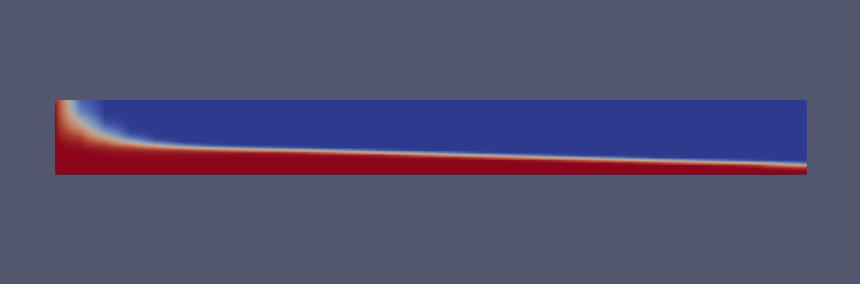
\includegraphics[width=0.6\linewidth]{fluido_mov1.png}
  \caption{Movimiento del fluido}
\end{figure}

\end{document}
